% XCircuit output "fte_12.tex" for LaTeX input from fte_12.eps
\def\putbox#1#2#3#4{\makebox[0in][l]{\makebox[#1][l]{}\raisebox{\baselineskip}[0in][0in]{\raisebox{#2}[0in][0in]{\scalebox{#3}{#4}}}}}
\def\rightbox#1{\makebox[0in][r]{#1}}
\def\centbox#1{\makebox[0in]{#1}}
\def\topbox#1{\raisebox{-0.60\baselineskip}[0in][0in]{#1}}
\def\midbox#1{\raisebox{-0.20\baselineskip}[0in][0in]{#1}}
   \scalebox{1}{
   \normalsize
   \parbox{6.69271in}{
   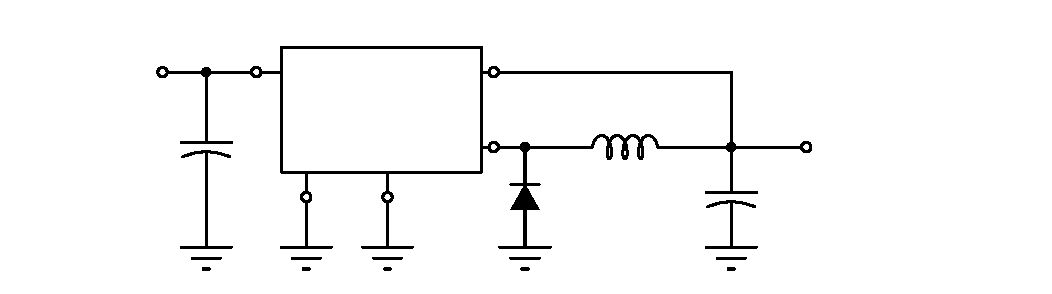
\includegraphics[scale=1]{fte_12}\\
   % translate x=712 y=188 scale 0.38
   \putbox{1.85in}{1.04in}{1.20}{LM2576-12}%
   \putbox{1.56in}{1.45in}{1.20}{1}%
   \putbox{3.56in}{0.49in}{1.20}{1N5822}%
   \putbox{3.72in}{1.04in}{1.20}{$100 \mu H$}%
   \putbox{5.01in}{0.45in}{1.20}{$1000 \mu F$}%
   \putbox{2.01in}{0.54in}{1.20}{3}%
   \putbox{2.60in}{0.54in}{1.20}{5}%
   \putbox{0.31in}{0.62in}{1.20}{$C_{in}$}%
   \putbox{0.31in}{0.37in}{1.20}{$100\mu F$}%
   \putbox{0.22in}{1.54in}{1.20}{$V_{in}$}%
   \putbox{3.14in}{1.45in}{1.20}{4}%
   \putbox{5.39in}{0.83in}{1.20}{12V Regulados}%
   \putbox{3.14in}{0.95in}{1.20}{2}%
   \putbox{3.35in}{1.49in}{1.20}{Realimetnacion}%
   \putbox{0.43in}{1.29in}{1.20}{30V }%
   \putbox{0.06in}{1.08in}{1.20}{No regulado}%
   } % close 'parbox'
   } % close 'scalebox'
   \vspace{-\baselineskip} % this is not necessary, but looks better
